\chap{Aku Mencari Tuhan Tanpa Kartu Pos} 

\begin{wrapfigure}[11]{l}{2.75cm}
\centering
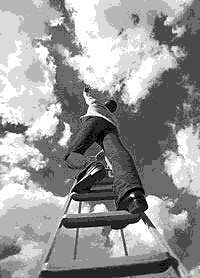
\includegraphics[scale=0.4]{gambar/aku-mencari-bw.jpg}
\end{wrapfigure}


Sebuah pesan di pintu mesin pendingin makanan. 
Tuhan pagi ini sengaja tak membangunkanku, ia hanya menempelkan secarik kertas:

"\textbf{ketika kau membaca ini, engkau telah terbangun}"


Lalu aku menuju meja makan, perut begitu lapar. Ketika aku membuka tudung saji, aku berharap Tuhan telah memasakkanku sepiring nasi goreng. Aku dapatkan secarik kertas di atas piring. Tertulis, "\textbf{ketika kau membaca ini, kau sudah kenyang}"

Di pintu lemari, akupun melihat sebuah kertas kecil, "\textbf{ketika kau membaca ini, hatimulah pakaianmu yang terindah}" Aku tahu, baju-bajuku telah membusuk di pojok kamar mandi.

Ketika aku membaca berbagai tulisan di dinding, laci, langit-langit dan pintu, tertulis, "\textbf{ketuklah, maka akan dibukakan}"

Ketika aku menyapa jalan, orang-orang yang berlalulalang, lampu merah dan asap-asap knalpot. Mereka lupa pada kata ``diam''. Melangkah seakan sudah menyatakan bahasa, bahwa mereka sedang diburu-buru hidup.

Aku mencari Tuhan tanpa kartu pos. Berharap Ia menuliskan pesan di badan bis-bis kota, di spanduk yang terbentang atau di kerumunan suara yang meneriakkan perutnya.

Aku mencari Tuhan dengan berkata-kata, dengan bertanya-tanya.
Aku mencari wajahnya dengan menatap mata-mata, senyum.
Aku menemukan jejaknya di sebuah sudut kota.

Kata mereka, “Tuhan pernah mampir dan selanjutnya pergi.”
"Mengapa tak kalian paksa saja ia tinggal di sini?"
"Kami rasa, masih banyak orang yang akan dijumpainya. Kami sudah kuat oleh kata-kata yang ditinggalkannya."

Aku terhenyak diam. Tuhan juga meninggalkanku pagi-pagi tadi.
Atau mungkin ia marah, ketika aku memperlakukannya tak pantas, memintanya untuk berjaga dikala tidur malamku bak seorang satpam, memintanya menghantarkanku selamat ke tujuan bagai seorang supir berpengalaman, meminta makanan, meminta rejeki, meminta jodoh, meminta naik pangkat, meminta \ldots meminta \ldots

"Di sini kami tak meminta. Karena kami tak mampu meminta padanya."

"Mengapa? Apakah kalian tak sadar, Ia mampu memberi apa yang kalian pinta."

"Kami tahu, Ia lebih tahu apa yang kami butuhkan. Tanpa diminta, Ia sudah melakukan.”

Ketika aku pulang tanpa bergandengan tangan dengan Tuhan, aku menemukan seseorang di bawah pohon sedang bernyanyi,

\begin{quote}
\textit{Berkat mu yang telah kuterima\\sempat membuatku terpesona\\
apa yang tak pernah kupikirkan\\itu yang kau sediakan bagiku\\siapakah aku ini Tuhan\\ jadi biji matamu\\dengan apakah kubalas Tuhan\\selain puji dan sembah kau \dots}
\end{quote}

Aku terdiam mendengarnya. Dingin bagai nisan yang kelak menuliskan namaku. Tuhan, maafkan bila aku selama ini membuatmu repot. Cukuplah firman-firman-Mu menjadi percakapan hatiku.

\begin{flushright}
\textit{Edisembiring\\15 July 2011}
\end{flushright}